%
% 14-integration.tex -- Integration der geometrischen Reihe
%
% (c) 2026 Prof Dr Andreas Müller
%
\subsection{Integration der geometrischen Reihe
\label{buch:analytisch:potenzreihen:subsection:integration}}
Durch Integration der geometrischen Reihe entlang einer Kurve
$\gamma$, die nicht geschlossen zu sein braucht, kann eine auf
dem Bild $\operatorname{im}\gamma = \gamma(I)$
definierte Funktion $g\colon\gamma(I)\to\mathbb{C}$ zu einer
Funktion $f(z)$ erweitert werden, die automatisch im holomorph und
analytisch ist.
Die Situation ist in Abbildung~\ref{buch:analytisch:fig:integral}
dargestellt.

\begin{satz}
Sei $\gamma\colon I\to\mathbb{C}$ eine differenzierbare Kurve und $g$
eine auf dem Bild $\operatorname{im}(\gamma)=\gamma(I)$ definierte 
stetige komplexe Funktion.
Dann ist die auf $\mathbb{C}\setminus\operatorname{im}\gamma$ definierte
Funktion
\begin{equation}
f(z)
=
\frac{1}{2\pi i}
\int_\gamma
\frac{g(x)}{x-z\mathstrut}\,dx
\end{equation}
holomorph.
\end{satz}

\begin{proof}
Da das Integrationsgebiet kompakt ist und $f$ stetig ist, kann unter
dem Integral differenziert werden.
Es ergibt sich die Ableitung
\begin{align*}
f'(z)
&=
\frac{1}{2\pi i}
\frac{d}{dz}
\int_\gamma
\frac{g(x)}{x-z\mathstrut}
\,dx
=
\frac{1}{2\pi i}
\int_\gamma
\frac{d}{dz}
\frac{g(x)}{x-z\mathstrut}
\,dx
=
\frac{1}{2\pi i}
\int_\gamma
\frac{g(x)}{(x-z\mathstrut)^2}
\,dx
\end{align*}
Insbesondere ist $f(z)$ komplex differenzierbar und damit $f$ holomorph.
\end{proof}

Andererseits kann man den Integranden mit der geometrischen Reihe
entwickeln und termweise integrieren.
%
% fig-integral.tex -- Integral der geometrischen Reihe
%
% (c) 2026 Prof Dr Andreas Müller
%
\begin{figure}
\centering
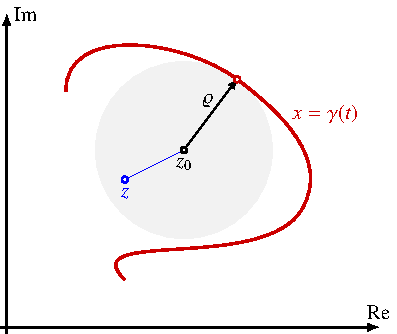
\includegraphics{chapters/040-analytisch/images/integral.pdf}
\caption{Durch Integration der geometrischen Reihe um den Punkte $z_0$
entlang eines nicht notwendigerweise geschlossenen Pfades $\gamma$ 
entsteht aus einer stetigen Funktion $g(x)$ auf der Kurve eine im
Komplement der Kurve holomorphe Funktion $f(z)$.
Um den Punkt $z_0$ kann für $f(z)$ eine eine Potenzreiheentwicklung 
angegeben werden kann, die als Konvergenzradius den minimalen
Abstand $\varrho$ zur Kurve hat.
\label{buch:analytisch:fig:integral}}
\end{figure}
%
Dazu verwenden wir
\eqref{buch:analytisch:eqn:geometrisch1}
und
\eqref{buch:analytisch:eqn:geometrischintegriert}
und erhalten
\begin{align}
f(z)
&=
\frac{1}{2\pi i}
\int_\gamma
\frac{g(x)}{x-z_0}
\cdot
\frac{1}{\displaystyle1-\frac{z-a\mathstrut}{x-a\mathstrut}}
\,dx
\notag
\\
&=
\frac{1}{2\pi i}
\int_\gamma
\frac{g(x)}{x-z_0}
\sum_{k=0}^\infty
\biggl(
\frac{z-z_0\mathstrut}{x-z_0\mathstrut}
\biggr)^k
\,dx
\notag
\\
&=
\sum_{k=0}^\infty
\biggl(
\frac{1}{2\pi i}
\int_\gamma
\frac{g(x)}{(x-z_0)^{k+1}}
\,dx
\biggr)
(z-z_0)^k.
\label{buch:analytisch:eqn:reihe}
\end{align}
Damit ist eine Potenzreihe im Punkt $a$ für die Funktion
$f(z)$ gefunden.
Sie ist konvergent, solange 
\[
\biggl|
\frac{z-z_0}{x-z_0}
\biggr|
=
\frac{|z-z_0|}{|x-z_0|}
<
1
\qquad\Rightarrow\qquad
|z-z_0| < |x-z_0|
\]
für alle $x$ entlang des Weges $\gamma$ gilt.
Dies wird erreicht, wenn 
\[
|z-z_0| < \inf_{\gamma} |x-z_0|,
\]
auf der rechten Seite steht der kleinste Abstand des Punktes $a$ vom
Weg $\gamma$.
Wir fassen dieses Resultat im folgenden Satz zusammen.

\begin{satz}
\label{buch:analytisch:potenzreihen:satz:integralanalytisch}
Sei $\gamma\colon I\to\mathbb{C}$ eine Kurve in $\mathbb{C}$ und
$f$ eine stetige Funktion auf dem Bild $\gamma(I)=\operatorname{im}\gamma$
der Kurve.
Dann ist die Funktion 
\begin{equation}
f(z)
=
\int_{\gamma} \frac{g(x)}{x-z}\,dx
\label{buch:analytisch:potenzreihen:eqn:fzintegral}
\end{equation}
analytisch und hat im Punkt $z_0 \in\mathbb{C}\setminus \operatorname{im}\gamma$
die Potenzreihenentwicklung
\[
f(z)
=
\sum_{k=0}^\infty
\biggl(
\frac1{2\pi i}
\int_\gamma \frac{g(x)}{(x-z_0)^{k+1}}\,dx
\biggr)
(z-z_0)^k
\]
mit Konvergenzradius
\[
\varrho(z_0)
=
\inf\{ |\gamma(t)-z_0|\mid t\in I\}.
\]
\end{satz}
